% Created 2014-07-17 Thu 09:54
\documentclass[11pt]{article}
\usepackage[latin1]{inputenc}
\usepackage{lmodern}
\usepackage[T1]{fontenc}
\usepackage{fixltx2e}
\usepackage{graphicx}
\usepackage{longtable}
\usepackage{float}
\usepackage{wrapfig}
\usepackage{rotating}
\usepackage[normalem]{ulem}
\usepackage{amsmath}
\usepackage{textcomp}
\usepackage{marvosym}
\usepackage{wasysym}
\usepackage{amssymb}
\usepackage{amsmath}
\usepackage[version=3]{mhchem}
\usepackage[numbers,super,sort&compress]{natbib}
\usepackage{natmove}
\usepackage{url}
\usepackage{minted}
\usepackage{underscore}
\usepackage[linktocpage,pdfstartview=FitH,colorlinks,
linkcolor=blue,anchorcolor=blue,
citecolor=blue,filecolor=blue,menucolor=blue,urlcolor=blue]{hyperref}
\usepackage{attachfile}
\author{John Kitchin}
\date{\today}
\title{org-to-word}
\begin{document}

\tableofcontents

\section{Pandoc does org-mode now}
\label{sec-1}

Pandoc (\url{http://johnmacfarlane.net/pandoc/}) is a document converter. It does a pretty good job of converting a document in one format to another. Pandoc also knows about org-mode now, and can convert an org-file to a Word document! We are going to test it out in this post to see what it does well with.

\subsection{A subsection with some equations}
\label{sec-1-1}

Einstein showed us that $E = mc^2$. 

A matrix looks like this:

\begin{equation}
\begin{matrix}
  a & b & c \\
  d & e & f \\
  g & h & i
 \end{matrix}
\end{equation}

\subsection{A section with a figure}
\label{sec-1-2}

Here is a figure in the document.

\begin{figure}[htb]
\centering
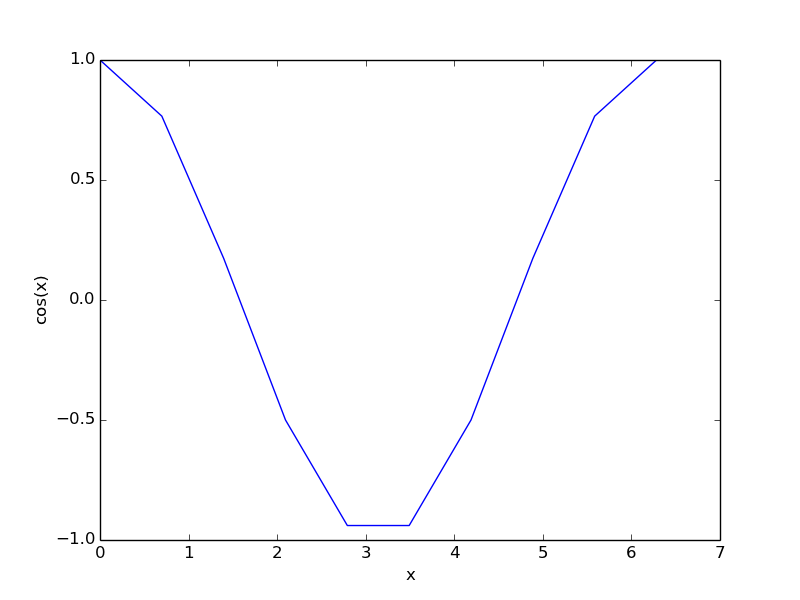
\includegraphics[width=.9\linewidth]{./images/cos-plot.png}
\caption{A cosine function.}
\end{figure}

\subsection{A section with a table}
\label{sec-1-3}

\begin{table}[htb]
\caption{A simple table.}
\centering
\begin{tabular}{rr}
x & y\\
\hline
1 & 1\\
2 & 4\\
3 & 9\\
\end{tabular}
\end{table}


\subsection{Some source code}
\label{sec-1-4}

Here is a python block.

\begin{minted}[frame=lines,fontsize=\scriptsize,linenos]{python}
print 'Hello Pandoc'
\end{minted}

\begin{verbatim}
Hello Pandoc
\end{verbatim}

And finally, we write a block that will convert this file to a Word document.

\begin{minted}[frame=lines,fontsize=\scriptsize,linenos]{common-lisp}
(save-buffer)
(shell-command "pandoc -s -S org-to-word.org -o org-to-word.docx")
\end{minted}

\begin{verbatim}
0
\end{verbatim}

Now, here is that \url{org-to-word.docx}

It is pretty good. The matrix

\bibliography{../../bibliography/references}
% Emacs 24.4.50.1 (Org mode 8.2.6)
\end{document}
